% Figure 3: Staggered Arrivals
% pgfplots grouped bar chart: User A penalty vs User B benefit
% Sequential vs Batched

\begin{figure}[t]
\centering
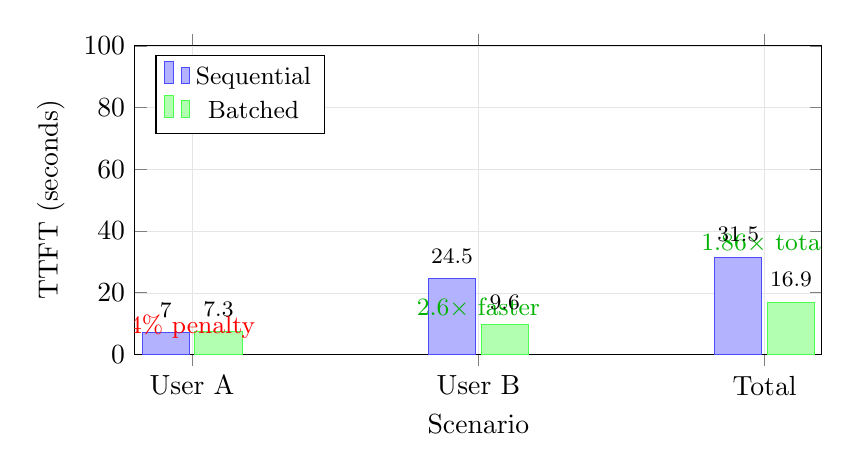
\begin{tikzpicture}
\begin{axis}[
    width=0.85\linewidth,
    height=5.5cm,
    ybar,
    bar width=0.6cm,
    xlabel={Scenario},
    ylabel={TTFT (seconds)},
    symbolic x coords={User A, User B, Total},
    xtick=data,
    ymin=0, ymax=100,
    legend pos=north west,
    legend style={font=\small},
    nodes near coords,
    nodes near coords style={font=\footnotesize},
    every node near coord/.append style={
        anchor=south,
        yshift=2pt
    },
    grid=major,
    grid style={line width=.1pt, draw=gray!20},
]

% Sequential serving
\addplot[fill=blue!30, draw=blue!70] coordinates {
    (User A, 7.0)
    (User B, 24.5)
    (Total, 31.5)
};
\addlegendentry{Sequential}

% Batched serving
\addplot[fill=green!30, draw=green!70] coordinates {
    (User A, 7.3)
    (User B, 9.6)
    (Total, 16.9)
};
\addlegendentry{Batched}

% Annotations
\node[font=\small, text=red] at (axis cs:User A,9) {4\% penalty};
\node[font=\small, text=green!70!black] at (axis cs:User B,15) {2.6$\times$ faster};
\node[font=\small, text=green!70!black] at (axis cs:Total,36) {1.86$\times$ total};

\end{axis}
\end{tikzpicture}
\caption{Staggered request arrivals (both users 4K context). User A submits at t=0, User B at t=2s. Sequential serving forces User B to wait for User A's completion (24.5s TTFT). Batched serving provides 2.6$\times$ speedup for User B at minimal cost to User A (4\% penalty). Net total TTFT improves 1.86$\times$.}
\label{fig:staggered}
\end{figure}
